\documentclass[journal]{IEEEtran}
\usepackage[a5paper, margin=10mm]{geometry}
%\usepackage{lmodern} % Ensure lmodern is loaded for pdflatex
\usepackage{tfrupee} % Include tfrupee package

%iffalse
\let\negmedspace\undefined
\let\negthickspace\undefined
\usepackage{gvv-book}
\usepackage{gvv}
\usepackage{cite}
\usepackage{amsmath,amssymb,amsfonts,amsthm}
\usepackage{algorithmic}
\usepackage{graphicx}
\usepackage{textcomp}
\usepackage{xcolor}
\usepackage{txfonts}
\usepackage{listings}
\usepackage{enumitem}
\usepackage{mathtools}
\usepackage{gensymb}
\usepackage{comment}
\usepackage[breaklinks=true]{hyperref}
\usepackage{tkz-euclide} 
\usepackage{listings}                                        
%\def\inputGnumericTable{}                                 
\usepackage[latin1]{inputenc}                                
\usepackage{color}                                            
\usepackage{array}                                            
\usepackage{longtable}                                       
\usepackage{calc}                                             
\usepackage{multirow}                                         
\usepackage{hhline}                                           
\usepackage{ifthen}                                           
\usepackage{lscape}
\usepackage{tabularx}
\usepackage{array}
\usepackage{float}
\usepackage{multicol}

\newcommand{\BEQA}{\begin{eqnarray}}
\newcommand{\EEQA}{\end{eqnarray}}
%\newcommand{\define}{\stackrel{\triangle}{=}}

\setlength{\headheight}{1cm} % Set the height of the header box
\setlength{\headsep}{0mm}     % Set the distance between the header box and the top of the text

%\usepackage[a5paper, top=10mm, bottom=10mm, left=10mm, right=10mm]{geometry}


\setlength{\intextsep}{10pt} % Space between text and floats

% Marks the beginning of the document
\begin{document}
\onecolumn
\bibliographystyle{IEEEtran}
\vspace{3cm}

%\renewcommand{\theequation}{\theenumi}
\numberwithin{equation}{section}
\numberwithin{figure}{section}
% \renewcommand{\thefigure}{\theenumi}
\renewcommand{\thetable}{\theenumi}

\title{Affine Transformations}
\author{EE24BTECH11059 -  Y SIDDHANTH}
\maketitle

% \renewcommand{\thefigure}{\theenumi}
\renewcommand{\thetable}{\theenumi} 

\setcounter{section}{1}
\textbf{Question: } Plot the ellipse whose focus is $\myvec{1 \\ -1}$, directrix $x-y-3 = 0$, and $e = \frac{1}{2}$. Plot the corresponding standard ellipse in the same graph using Affine Transformation.

\bigskip

\textbf{Solution: } 
\begin{table}[h!]    
	\centering
	

	\caption{Variables Used}
	\label{tab1-1.9-6}
\end{table}\\

First we find the $V, u, f$ for the actual ellipse using the following formulas: 
\begin{align}
	\vec{V} &=\norm{\vec{n}}^2\vec{I}-e^2\vec{n}\vec{n}^{\top}, 
	\\
	\vec{u} &= ce^2\vec{n}-\norm{\vec{n}}^2\vec{F}, 
	\\
	f &= \norm{\vec{n}}^2\norm{\vec{F}}^2-c^2e^2
\end{align}

Upon solving, we get:
\begin{align}
	\vec{V} &= \myvec{\frac{7}{4} & \frac{1}{4} \\ \frac{1}{4} & \frac{7}{4}} ,
	\\
	\vec{u} &=\frac{5}{4}  \myvec{ -1 \\ 1}
	\\
	f &= \frac{7}{4}
\end{align}

For Affine Transformation, we have to spectral / eigen decompose the matrix $\vec{V}$. \\ 

\begin{align}
	\vec{V} = \vec{P}\vec{D}\vec{P^\top}
\end{align}
To find $\vec{D}$, we will have to find the eigen values of the matrx $\vec{V}$.

	\begin{align}
		|\vec{V}  - \lambda\vec{I}|  &= 0,\\
		|\vec{V}  - \lambda\vec{I}|  &= \mydet{\frac{7}{4} - \lambda& \frac{1}{4}\\ \frac{1}{4} & \frac{7}{4} - \lambda}\\
		\lambda_1, \lambda_2 &= 2 , \frac{3}{2} \\
		\therefore 	\vec{D} &= \myvec{2 & 0 \\ 0 & \frac{3}{2}} , \label{Ddef}
	\end{align}
Note: In \eqref{Ddef}, the order of the eigen values that I have chosen is random but once a certain order has been set for the eigen values, then that order must be followed throughout the procedure. \\
\\
Now, to find $\vec{P}$ which is the matrix containing the normalised eigen vectors. So we have to find the eigen-values.



\begin{align}
	\vec{V}\vec{p_2^\prime} &= \lambda_2 \vec{p_2^\prime} \\
	\myvec{\frac{7}{4} & \frac{1}{4} \\ \frac{1}{4} & \frac{7}{4}} \vec{p_2^\prime}  &= 2\vec{p_2^\prime} \\
\end{align}
Taking an augmented matrix,
\begin{align}
	\brak{
	\begin{array}{cc|c}
		\frac{7}{4} - \lambda_2 & \frac{1}{4} & 0\\ 
		\frac{1}{4} & \frac{7}{4} - \lambda_2& 0
	\end{array}}\vec{p_2^\prime}  &=  \myvec{0 \\ 0} 
\end{align}
\begin{align}
	\brak{
	\begin{array}{cc|c}
		\frac{1}{4} & \frac{1}{4} & 2\\ 
		\frac{1}{4} & \frac{1}{4} & 2
	\end{array}}
	\xleftrightarrow[]{R_1 \leftarrow {4 R_1}}
	\xleftrightarrow[]{R_2 \leftarrow {R_2-\frac{1}{4}R_1}}
	\brak{
	\begin{array}{cc|c}
		1 & 1 & 0\\ 
		0 & 0 & 0
		\end{array}}
\end{align}
If we take $\vec{p_2^\prime}  = \myvec{p_{21}^\prime \\ p_{22}^\prime}$, and put in the above equation, we get,
\begin{align}
	\vec{p_2^\prime} = p_{21}^\prime \myvec{-1 \\ 1} \implies \vec{p_2^\prime} =  \myvec{-1 \\ 1}
\end{align}
$\therefore \vec{p_2^\prime}  = \myvec{-1 \\ 1} \implies \vec{p_2} = \frac{\vec{p_2^\prime} }{\norm{\vec{p_2^\prime}}}  = \myvec{ -\frac{1}{\sqrt{2}} \\ \frac{1}{\sqrt{2}}}$ \\
Similarly solving for $\vec{p_1^\prime}$ , we get,

\begin{align}
	\vec{p_1^\prime} &=  \myvec{1 \\ 1} \\
\end{align} 
$\therefore \vec{p_1^\prime}  = \myvec{1 \\ 1} \implies \vec{p_1} = \frac{\vec{p_1^\prime} }{\norm{\vec{p_1^\prime}}}  = \myvec{ \frac{1}{\sqrt{2}} \\ \frac{1}{\sqrt{2}}}$ \\
By definition $\vec{P} = \sbrak{\vec{p_1} ~ \vec{p_2}}$ \\ 

\begin{align}
	\vec{P} = \myvec{ \frac{1}{\sqrt{2}} & -\frac{1}{\sqrt{2}} \\ \frac{1}{\sqrt{2}} & \frac{1}{\sqrt{2}} } \label{Rdef}
\end{align}

Now, we will use Affine Transformations to get the standard ellipse equation.

\begin{align}
	\vec{y}^\text{T}\brak{\frac{\vec{D}}{f_0}}\vec{y} &= 1\\
	\vec{x} &= \vec{Py} + \vec{c} \label{t1}\\
\end{align}

Where 

\begin{align}
	f_0 &= \vec{u}^\text{T}\vec{V}^{-1}\vec{u} - f  = \frac{25}{4} \myvec{-1 & 1} \myvec{\frac{7}{12} & \frac{-1}{12} \\ \frac{7}{12} & \frac{-1}{12}}  \myvec{-1 \\ 1}  - \frac{7}{4}= \frac{25}{12} -  \frac{7}{4} = \frac{1}{3}\\
	\vec{c} &= -\vec{V}^{-1}\vec{u} = -\frac{5}{4}  \myvec{-1 & 1} \myvec{\frac{7}{12} & \frac{-1}{12} \\ \frac{7}{12} & \frac{-1}{12}}\myvec{ -1 \\ 1} = \frac{5}{6}  \myvec{ 1 \\ -1}
\end{align}

Finally, we get the standard form of the ellipse.

\begin{align}
		\vec{y}^\text{T}\myvec{2 & 0 \\ 0 & \frac{3}{2}}\vec{y} &= \frac{1}{3}
\end{align}
Plotting the standard and the actual ellipse using python,

\begin{figure}[H]
	\centering
	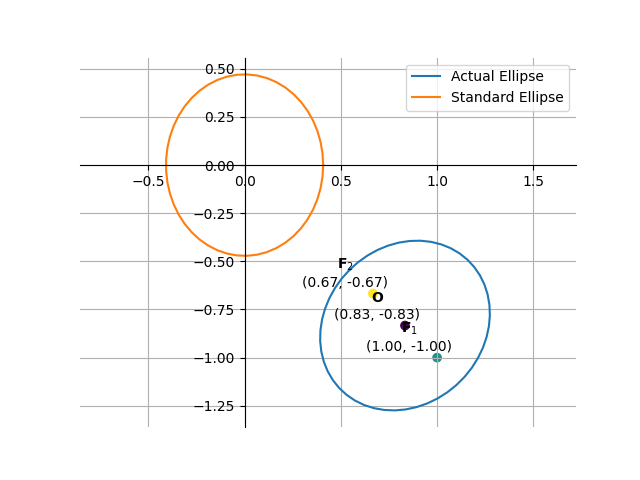
\includegraphics[width=0.75\columnwidth]{Figures/fig1.png} 
	\caption{}
	\label{fig1}
\end{figure} 

Code for Figure \ref{fig1} can be found at:
\begin{lstlisting}
codes/misc.py
\end{lstlisting}

\end{document}